\documentclass[conference]{IEEEtran}
\usepackage[utf8]{inputenc}

%\usepackage[portuguese]{babel}
%
%\usepackage{glossaries}  
%\setacronymstyle{short-long}
%
%\newacronym{mpls}{MPLS}{Multiprotocol Label Switching}
%\newacronym{asic}{ASIC}{Application-specific Integrated Circuit}
%
%\makeglossaries

\usepackage[pdftex]{graphicx}
\graphicspath{{./Imagens/}}

% correct bad hyphenation here
\hyphenation{op-tical net-works semi-conduc-tor DEFCON}
%

\begin{document}
\title{Wireless Personal Area Networks\\
  \large Redes de Comunicações Móveis\\
  2016/2017
}

\author{\IEEEauthorblockN{Fábio Teixeira}
\IEEEauthorblockA{Faculdade de Ciências da\\Universidade do Porto\\Email: up201305725@fc.up.pt}
\and
\IEEEauthorblockN{Vanessa Silva}
\IEEEauthorblockA{Faculdade de Ciências da\\Universidade do Porto\\Email: up201305731@fc.up.pt}
}

\maketitle

% As a general rule, do not put math, special symbols or citations
% in the abstract
\begin{abstract}
Resumo aqui.
\end{abstract}


\IEEEpeerreviewmaketitle


\section{Introdução}
Introdução aqui.
%WPANs faz parte do grupo das tecnologias da área sem fio e são particularmente aplicáveis em aplicações que exigem baixa taxa de transferência de dados, um alcance limitado, baixo consumo de energia e que exigem que os dispositivos sejam fisicamente pequenos e de baixo custo. (A REVIEW OF WPAN SECURITY: ATTACKS AND PREVENTION)

%Uma rede de área pessoal (PAN) distingue-se de outros tipos de redes de dados em tamanho e escopo. As comunicações em PANs são normalmente confinadas a uma pessoa ou objeto que tipicamente se estende até 10 metros em todas as direções e envolve dois ou mais objetos ou pessoas, tanto estacionários como em movimento. [cite: WIRELESS PERSONAL AREA NETWORKS: AN OVERVIEW OF THE IEEE P802.15 WORKING GROUP]
%Uma rede de área pessoal sem fio (WPAN) é um sistema de comunicação de dados ad hoc sem fio que permite que vários dispositivos de dados independentes se comuniquem. 


\section{Conceito, Motivação, Objetivos, Benefícios}

\subsection{Conceito}

Uma \textit{Wireless Personal Area Network} (WPAN) é uma rede de área pessoal (\textit{Personal Area Network} (PAN)) que permite conectar dispositivos, (como PCs, PDAs, telemóveis e impressoras), centrados na área (curta) de uma pessoa, com base em conexões sem fio (\textit{Wireless}). Deste modo, WPAN forma uma "bolha" wireless em torno de uma pessoa, conhecida como \textit{Personal Operating Space} (POS) \cite{prasad2004ofdm}, e essa bolha pode, dinamicamente, expandir-se e contrair-se consoante as necessidades.

Além da conexão entre os dispositivos pessoais, que formam a bolha, WPANs devem fornecer ao utilizador uma conexão \textit{ad hoc} (\ref{redes_ad_hoc}) com os recursos e aplicações compatíveis que entram no seu POS \cite{prasad2004ofdm}.
Esta permite que os dispositivos pessoas se comuniquem com outros dispositivos em que a faixa de comunicação interceta o seu POS.

O paradigma das comunicações tradicionais destina-se a estabelecer ligações de comunicação entre dispositivos, enquanto que as WPANs destinam-se a estabelecer comunicações entre pessoas, (dispositivos pessoais habilitados para comunicação), e recursos funcionais/dados através de um meio sem fios (substituindo o tradicional "cabo").

As \textit{Wireless Personal Area Networks} são projetadas para operarem na banda mundial ISM (\textit{Industrial}, \textit{Scientific} e \textit{Medical}) de 2,4 GHz. Esta banda proporciona disponibilidade geral em todo o mundo e adequação a soluções de rádio de baixo custo, baixo consumo de energia, curto alcance e não exige a necessidade de uma licença, usando uma técnica FHSS (\textit{Frequency Hopping Spread Spectrum}). Essa última é baseada na especificação do Bluetooth \ref{bluetooth}, no qual se tornou um padrão IEEE denominado de 802.15 WPANs. %[cite: OPTIMIZING THE TOPOLOGY OF BLUETOOTH WIRELESS PERSONAL AREA NETWORKS e WIRELESS PERSONAL AREA NETWORKS: AN OVERVIEW OF THE IEEE P802.15 WORKING GROUP]


\subsection{Motivação}

A motivação para tais redes vem da necessidade da troca de dados não só em grandes distâncias (que é tradicionalmente referida como comunicações), mas também entre pessoas que estão em uma "conversação" em uma curta distância (normalmente até um limite de 10 metros), assim como da necessidade dessa troca de dados ser realizada em um meio sem fios.


\subsection{Objetivos}

Os principais objetivos das WPANs são \cite{prasad2004ofdm}:

\begin{itemize}

 \item Baixo consumo de energia - problema crítico, dado que a velocidade com que o desempenho da bateria melhora é bastante lenta, em comparação com o explosivo crescimento das comunicações sem fio;
 \item Operação no espectro não licenciado - WPANs usam ligações sem fio não licenciadas, uma vez que esta é a única forma de conseguirem conectividade onipresente sem impacto adverso em uma infraestrutura sem fio existente;
 \item Baixo custo;
 \item Pequeno tamanho de pacote.
 
\end{itemize}

\subsection{Benefícios}

%Livro:  A conectividade ad hoc proporcionada pelas WPANs pode motivar o design dos próprios dispositivos de computação, bem como a distribuição das tarefas e capacidades de computação em diferentes dispositivos.


\section{Funcionamento, Hardware}

\subsection{Funcionamento}

Uma WPAN deve suportar as seguintes operações (inter-relacionadas) \cite{prasad2004ofdm}:

\begin{itemize}

 \item Descoberta de serviço, ou seja, os dispositivos devem ter a capacidade de descobrirem o recurso de serviço ou informação necessária;
 \item Estabelecimento de conexão \textit{ad hoc}, ou seja, os dispositivos devem ter a capacidade de estabelecerem uma conexão \textit{ad hoc} com o dispositivo que oferece esse serviço ou contém esse recurso.
 
\end{itemize}

A descoberta de serviço permite que um dado dispositivo de computação tenha acesso ao serviço que está disponível dentro do seu intervalo de comunicação.
Por exemplo, um dado PDA, (\textit{Personal Digital Assistants}), encontra uma impressora dentro do seu intervalo de comunicação, reconhece-o, (descoberta de serviço), como um recurso de computador disponível (desde que certas condições de segurança sejam satisfeitas) e usa-o, (estabelecimento de conexão), como se a impressora fosse instalada no seu \textit{software} \cite{prasad2004ofdm}.

\subsection{Redes \textit{Ad Hoc}} \label{redes_ad_hoc}

Uma rede \textit{ad hoc} é um tipo de rede sem fio constituída por nós (ou estações) que cooperam entre si de forma a encaminharem pacotes na rede (determinam quando um nó (ou estação) pode transmitir e receber dados), sem a necessidade de uma infraestrutura. Cada nó (ou estação) pode comunicar-se diretamente com outro nó (ou estação). [DISTRIBUTED TOPOLOGY CONSTRUCTION OF BLUETOOTH WIRELESS PERSONAL AREA NETWORKS e Qualidade de Serviço em Redes 802.11] 
Esta comunicação (de um nó A para um nó B) só pode ser estabelecida se o nó B estiver dentro do raio de ação (locais onde o sinal chega com clareza) de A ou então, se existir um ou mais nó entre A e B que possam encaminhar os dados.

Em termos de roteamento, toda a rede é baseada na ideia de que os dispositivos funcionarem tanto como \textit{routes} e como \textit{hosts} \cite{prasad2004ofdm}.

O principal problema que se encontra neste tipo de redes é a conceção de relações confiáveis entre as chaves criptográficas públicas sem o auxílio de um reconhecimento confiável de terceiros. 
Existem outros problemas associados, como por exemplo, o “ataque de exaustão de bateria” como uma forma especial de ataque de negação de um dado serviço \cite{prasad2004ofdm}.



\subsection{Hardware - Tecnologias Associadas}

Existem várias tecnologias \textit{standard} que fornecem conectividade sem fio em curtas distâncias. Neste artigo vamos destacar as seguente, \textbf{Bluetooth}, \textbf{IrDA}, \textbf{Zigbee}, \textbf{HomeRF} e \textbf{UWB}.
Embora cada uma destas tecnologias tenha atingido aplicações e modelos de uso diferentes, o princípio por detrás de todas é a utilização de algum tipo de tecnologia de rádio subjacente, de forma a permitir a transmissão wireless de dados, fornecer suporte para a formação de redes e gerenciar vários dispositivos através de \textit{software} de alto nível \cite{prasad2004ofdm}.

\section{Modelos de Arquitetura/\textit{standard}}

\subsection{Bluetooth} \label{bluetooth}

O Bluetooth, também conhecido por IEEE 802.15.1, é um tipo de tecnologia WPAN sem fios, que estabelece uma comunicação de curta distância e baixo custo. 
Tem como objetivo o estabelecimento de conexões e troca de informação entre dispositivos, como telemóveis, computadores, impressoras, câmaras e até consolas de jogos, utilizando para isso uma frequência de rádio de curto alcance. 
Foi lançado em 1994 pela Ericsson, embora outras companhias como a Nokia, a IBM, a Intel e a Toshiba também se tenham juntado à empresa sueca em 1998, formando um grupo chamado Bluetooth SIG (\textit{Special Interest Group}), com o intuito de desenvolver, promover e expandir esta tecnologia. 
Nos dias de hoje, milhares de empresas já se juntaram ao grupo, entre elas estão nomes fortes como a Samsung, a Microsoft, a Motorola, a Dell, a HP, a Phillips, a Siemens e a Texas.

Algumas das especificações desta importante tecnologia são:

\begin{itemize}

 \item Não requer obrigatoriamente linha de vista para funcionar, sendo capaz de comunicar através de barreiras físicas, como é o caso da tecnologia de infravermelhos.
 \item Conta tipicamente com um alcance de 10 metros, (alcance das WPANs), embora este valor possa ser amplificado. 
 \item Opera na faixa de licença-livre ISM (Industrial, Scientific, Medical) a aproximadamente 2,45 GHz, com um débito máximo típico de 1 Mbps, que se estima que possa ser aumentado, com futuras especificações.
 \item O protocolo Bluetooth divide ainda a faixa de 2,45 GHz em 79 canais e muda de canal cerca de 1600 vezes por segundo, de forma a evitar possíveis interferências com outros protocolos que usem a mesma faixa.

\end{itemize}

\subsubsection{Funcionamento}

\begin{figure}[!t]
  \centering
  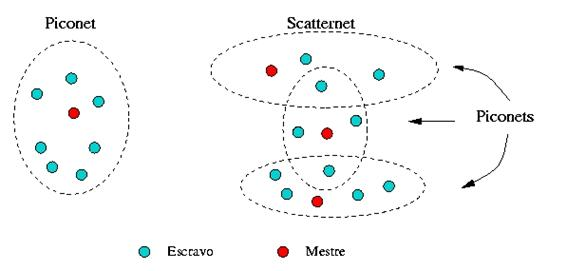
\includegraphics[width=0.45\textwidth]{Esquema_Bluetooth.png}
  \caption{Topologia da tecnologia Bluetooth \cite{blueesptec}.}
  \label{fig:topBluet}
\end{figure}

\begin{figure}[!t]
  \centering
  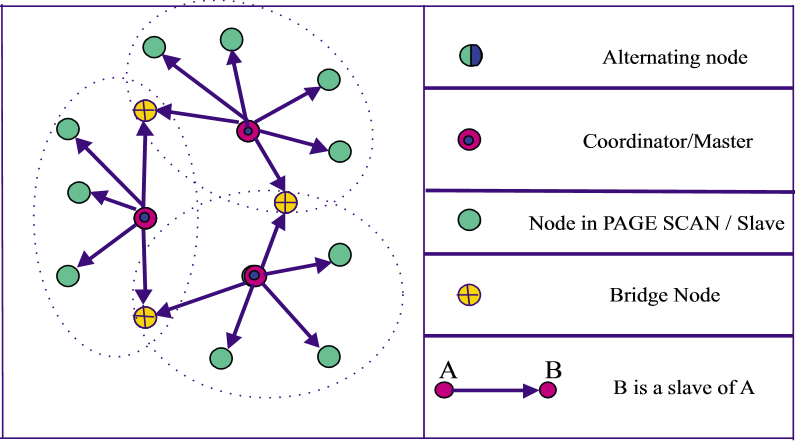
\includegraphics[width=0.45\textwidth]{no_ponte.png}
  \caption{Representação da conexão de três \textit{piconets} atavés de um nó ponte \cite{salonidis2005distributed}.}
  \label{fig:noPonte}
\end{figure}

O Bluetooth baseasse numa camada física de saltos de frequência, que permite que dispositivos portáteis formem redes \textit{ad hoc} sem fio de curto alcance. 
Os \textit{hosts} Bluetooth não são capazes de comunicar a menos que se tenham previamente descoberto uns aos outros, através da sincronização dos seus padrões de tempo e frequência. 
Assim, mesmo que todos os nós estejam próximos uns dos outros, apenas os nós que estão sincronizados com o transmissor podem ouvir a transmissão. 
Para suportar comunicação \textit{any-to-any}, os nós devem ser sincronizados de modo a que os pares de nós, que se podem comunicar uns com os outros, formem um gráfico conectado.

O sistema de saltos de frequência, em que o Bluetooth se baseia, define vários canais para comunicação, sendo que cada canal é baseado numa sequência de salto de frequência diferente. 
Assim, um grupo de dispositivos que compartilham um mesmo canal é chamado de \textit{piconet}. 

Cada \textit{piconet} tem uma unidade \textbf{mestre} (\textit{master}) que seleciona uma sequência de salto de frequência para o \textit{piconet} e controla o acesso ao canal. 
Os outros participantes do grupo, conhecidos como unidades \textbf{escravas} (\textit{slaves}), são sincronizados com a sequência de salto do \textit{piconet master}. 

Dentro de um \textit{piconet}, o canal é compartilhado usando um \textit{slotted Time Division Duplex} (TDD), em que um mestre usa um protocolo de pesquisa para alocar faixas horárias para os nós escravos. O número máximo de escravos que podem ser simultaneamente ativos num \textit{piconet} é sete. 

Quando os vários \textit{piconets} (lado esquerdo da figura (\ref{fig:topBluet})) são conectados, forma-se uma rede wireless chamada \textit{scatternet}, como ilustrado à direita da figura (\ref{fig:topBluet}).
Isto é possível, pois cada \textit{piconet} utiliza uma sequência de salto diferente, o que faz com que múltiplos \textit{piconets} possam coexistir numa área comum. 
Estes são então conectados através de uns nós especiais, chamados de nós \textbf{ponte}, que podem ser construídos entre dois nós mestre, como podemos ver na figura (\ref{fig:noPonte}), entre um nó mestre e um escravo ou entre dois nós escravos. 

Dada uma coleção de dispositivos Bluetooth, é necessário um protocolo explícito de construção de topologia para formar \textit{piconets}, atribuir escravos a \textit{piconets} e conectar \textit{piconets} através de nós ponte, de modo que o \textit{scatternet} resultante fique conectado. Tal protocolo deve ser assíncrono, distribuído e pode começar com nós que não têm qualquer informação sobre o seu ambiente.

\subsubsection{Benefícios}

Com o Bluetooth as conexões através de cabos tenderão a desaparecer, o que evita o problema da interligação dos cabos de conexão, que muitas vezes não são compatíveis com certos equipamentos. 
A tecnologia direciona-se para um maior aproveitamento das capacidades de conectividade, podendo-se envolver todos os equipamentos de uma pequena área (fixos e móveis) para interagirem entre si. 

O consumo de cada transmissor Bluetooth é de aproximadamente 50 mA, dentro do limite de 10 metros, o que representa cerca de 3\% do consumo total de um telemóvel, valor que é quase irrisório comparado com outras tecnologias sem fios. 
Este baixo consumo permite que os dispositivos venham já com a tecnologia de fábrica, sem comprometer a autonomia das baterias. 
Os \textit{developers} do projeto depressa perceberam que muito mais seria possível fazer aproveitando a tecnologia do Bluetooth. 
Se transmitir informação entre um computador e uma impressora era uma realidade, também o poderia ser transmitir dados de um telemóvel para uma impressora, ou mesmo entre impressoras. 
E com o baixo custo de um chip Bluetooth (cerca de 5 euros) e o baixo consumo de energia da tecnologia. O número de aplicações e benefícios da tecnologia rapidamente se tornaram inimagináveis.

\subsubsection{Classes e Versões}

O Bluetooth possibilita a comunicação entre dispositivos enquanto estão dentro do raio de alcance. Os dispositivos não precisam de estar em linha de vista um do outro, desde que a transmissão recebida tenha a potência suficiente para a comunicação via rádio funcionar.

Existem atualmente 3 classes da tecnologia, numeradas de 1 a 3. A classe 1 é a mais potente, permitindo consumos até 100 mW com um alcance de 100 metros. A classe 2, por seu lado, possibilita cerca de 2.5 mW de potência máxima, com um alcance de 10 metros. Já a classe 3 permite 1 mW de potência, transmitindo numa distância de cerca de 1 metro.

Versões também exisitam 3 até há pouco tempo, mas recentemente foi lançado o Bluetooth 4, que traz vantagens no consumo de energia, velocidade e segurança, entre outros. A versão 3 era até então a versão com maior taxa de transmissão - cerca de 24 Mbits/s -, enquanto que as versões 2 e 1.2 se ficavam pelos 3 e 1 Mbits por segundo, respetivamente.

\subsubsection{Bluetooth vs. Wi-Fi}

Resumidamente, embora o Bluetooth utilize a mesma banda de 2,45 GHz do 802.11b e do 802.11g, o Wi-Fi continua a ser uma melhor opção, já que uma rede Bluetooth é muito mais lenta e, para além de suportar poucos dispositivos, é ainda menos segura. O Wi-Fi, por sua vez, apesar de requerer mais configurações, é melhor para operar redes de alta-escala pelo simples facto de suportar conexões rápidas e seguras com melhor potência de transmissão e receção.

\subsection{IrDA}

\subsection{IEEE 802.15.4 - Zigbee}

%Em março de 1999, o Comitê de Normas de Rede Local e Metropolitana IEEE 802 formou um novo Grupo de Trabalho para desenvolver padrões de comunicação para redes de área pessoal sem fio para dispositivos de computação portáteis e móveis. O novo grupo é designado Grupo de Trabalho do Projeto 802.15 para Redes Pessoais Sem Fio (WPANs). [cite: WIRELESS PERSONAL AREA NETWORKS: AN OVERVIEW OF THE IEEE P802.15 WORKING GROUP]


\subsection{HomeRF}

\subsection{UWB - Ultra-wideband}


%Exemplo de imagem em latex em duas colunas
%\begin{figure}[!t]
%  \centering
%  \includegraphics[width=0.45\textwidth]{switch_openflow.png}
%  \caption{Switch OpenFlow dedicado \cite{xia2015survey}.}
%  \label{fig:refswitchOP}
%\end{figure}

%Exemplo de referencia à imagem
%\ref{fig:refswitchOP}


\section{Conclusões}
Conclusões aqui.

\bibliography{ref}{}
\bibliographystyle{IEEEtran}

\end{document}
